\pagebreak
\chapter{Data Acquisition and Manipulation}
\label{sec:data}

\section{The Human Connectome Project \textit{(HCP)}}

\glsreset{T2w}
The data handled in this project has been amassed through the \gls{HCP}. The \gls{HCP} was an ambitious five-year effort to characterize brain connectivity and function and their variability in healthy adults. A consortium of investigators studied a population of 1200 subjects, using multiple imaging modalities along with extensive behavioral and genetic data. The imaging modalities included \gls{dMRI}, \gls{r-fMRI}, \gls{t-fMRI}, \gls{T1w} and \gls{T2w} \gls{MRI} for structural and myelin mapping, plus combined \gls{MEG} and \gls{EEG}. 

During the first phase, the WU-Minn \gls{HCP} consortium made a major effort to improve the methods of data acquisition and analysis, since up to that point in time, despite their great promise, all of the modalities that could be applied to \textit{in vivo} human \gls{connectomics} had serious limitations in their sensitivity, accuracy and resolution \cite{VanEssen2012}. This initial phase was followed by a three-year period of data acquisition from the main cohort \cite{HCP}.
% Describing the cohort subjects
A key objective was to understand inter-individual variability of brain circuits, including its genetic bases and its relation to behavior, rather than merely aiming to determine the average, or typical connectivity in healthy adults. This was achieved by sampling more than three hundred young adult sibships of average size 3-4, with most of these including a \gls{MZ} or \gls{DZ} twin pair. All subjects were between 22 and 35 years old, an age range chosen to represent healthy adults beyond the age of major neurodevelopmental changes and before the onset of neurodegenerative changes. While the \gls{HCP} was cross-sectional, many participants were drawn from ongoing longitudinal studies \cite{Sartor2011, Edens2010}; they had extensive previous assessment, particularly with respect to history of the presence or absence of emotional and behavioral problems. 

\begin{figure}[htbp]
    \centering
    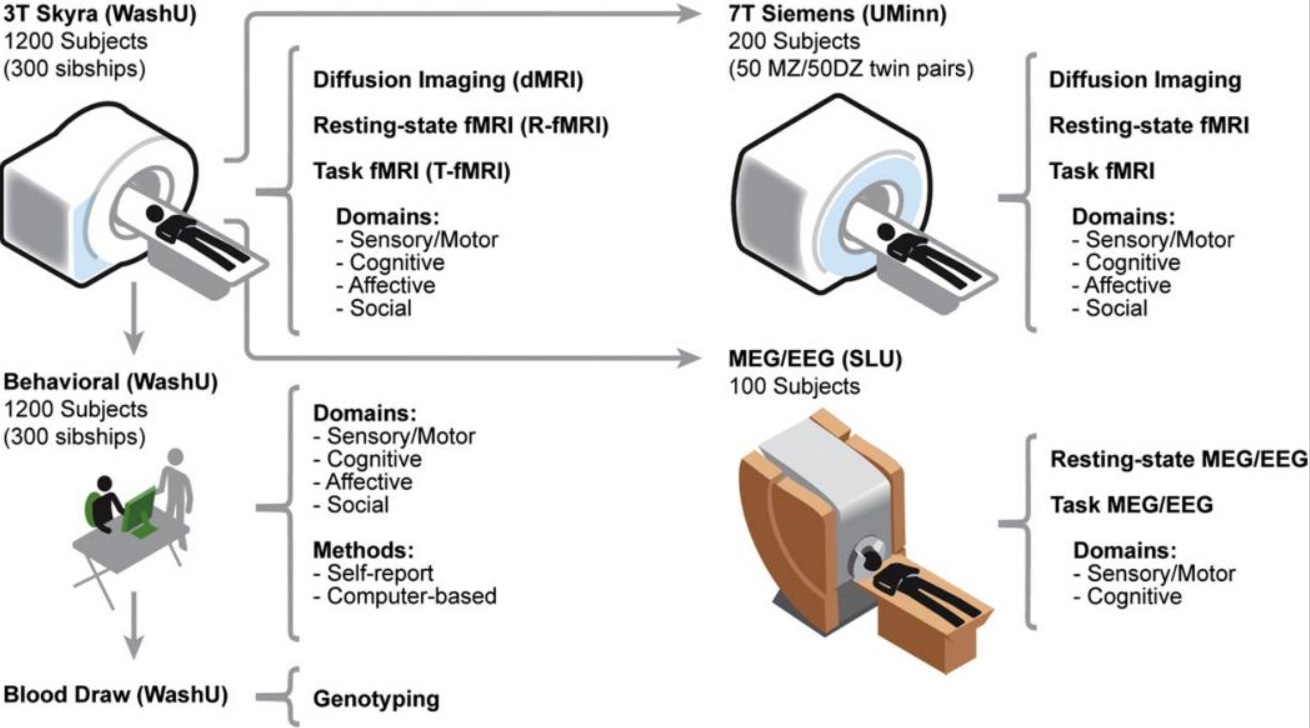
\includegraphics[width = 0.75\textwidth]{assets/images/HCP_plan.png}
    \caption[HCP Image Acquisition Schematic Summary]{Schematic summary for acquiring imaging, behavioral, and genetic data using \gls{MR} and \gls{MEG}/\gls{EEG} scanners at three \gls{HCP} sites. Adapted from \cite{HCP}.}
    \label{fig:HCP_plan}
\end{figure}

% Methods of HCP
As for the methods, \autoref{fig:HCP_plan} provides a high-level view of the plans used for data acquisition in Phase II of the project. Each subject spent two days at \gls{WashU} for: behavioral assessment, whose measures spanned a broad range in the domains of cognition, emotion, perception and motor function, and they were mainly drawn from the \gls{USA} \gls{NIH} but were supplemented by a number of complementary additional measures, blood draw for eventual genotyping, and four \gls{MR} scanning sessions, with three lasting one hour. The scans at \gls{WashU} were carried out using a customized \SI{3}{\tesla} connectome scanner adapted from Siemens Skyra, designed to improve the quality and resolution of connectivity data; a subset of 200 subjects was also scanned at \gls{UMinn} using a new \SI{7}{\tesla} system which offers advantages, especially for the resting and task-based fMRI studies, but also for diffusion-based techniques if sufficiently short echo times can be achieved for diffusion weighting. Both systems capitalized on major improvement in advanced \gls{MR} pulse sequences to obtain \gls{dMRI}, \gls{r-fMRI}, and \gls{t-fMRI}, plus \gls{T1w} and \gls{T2w} anatomical scans. The \gls{t-fMRI} scans included a range of tasks aimed at providing broad coverage of the brain and identifying as many functionally distinct domains and cortical parcels as possible. A subset of 100 subjects was also studied with combined \gls{MEG} and \gls{EEG} at \gls{SLU}, which offer much better temporal resolutions (\si{\milli\second} instead of \si{\second}) but lower spatial resolution than \gls{MR}. 

\subsection{Task-fMRI Battery of the HCP}

% Generic goal of HCP t-fMRI tasks
The \gls{HCP} used \gls{t-fMRI} to help delineate the relationships between individual differences in the neurobiological substrates of mental processing and both functional and structural connectivity \cite{Barch2013}. We know that there are important individual differences in suh patterns of connectivity even among persons with no diagnosable neurological or psychiatric disorders, and there is increasing evidence that this variability is associated with alterations in cognitive and behavioral variables that constrain real world function \cite{Basset2009, Song2008, Heuvel2009}. For example, higher \gls{IQ} among healthy adults is associated with shorter path length and higher global efficiency in measures of brain functional connectivity \cite{Li2009} as well as greater global connectivity in prefrontal cortex \cite{Cole2012}, thus providing evidence that more efficient connectivity contributes to more effective cognitive function. As another example, developmental research is increasingly suggesting that maturation of functional and structural networks in the human brain underlies key aspects of cognitive and emotional development \cite{Fair2007, Fair2009, Hwang2013, Imperati2011, Stevens2009, Supekar2009, Zuo2010}.

% What measures were assessed and what the task design and selection was based on
The goal for the \gls{HCP} was to identify and utilize a reliable and well-validated battery of measures that assess a wide range of human functions and behaviors in a reasonable amount of time (3-4\si{\hour}), to satisfy subject burden considerations. The base for the \gls{HCP}'s  assessment was the set tools and methods developed by the \gls{NIH} Toolbox of Assessment of Neurological and Behavioral function \cite{NIH_Toolbox}, including tasks developed and validated using item response theory and computer adaptive testing where appropriate and feasible. The battery was additionally expanded with tests to include measures of the following domains not covered by the Toolbox: 1) subthreshold symptoms of mood, anxiety and substance abuse; 2) additional measures of visual, memory and emotion processing; 3) personality; 4) delay discounting, as a measure of self-regulation and neuroeconomic decision-making \cite{Dalley2008, Shamosh2008}; 5) fluid intelligence as a measure of higher-order relational reasoning that has been linked to important individual differences in both life function and brain function \cite{Burgess2011}; 6) menstrual cycle and hormonal function for women; and 7) sleep funciton, which may be highly relevant to understanding individual differences in behavior.

% Goal of the tasks
The choice of \gls{t-fMRI} tasks was driven by the following considerations. The aim was to identify nodes: 1) in well-characterized neural systems; 2) in as wide a range of neural systems as possible; 3) with activation locations that are reliable over time in individual subjects; 4) with activations consistently detectable in most individuals (sensitivity); and 5) that are associated with a broad range of cognitive and affective processes of interest to the \gls{NIH} Blueprint Institutes. In addition, it was necessary that a subset of the tasks must be suitable for \gls{T-MEG}.

% Domains the tasks cover
Initial piloting targeted a broad range of domains that sampled diverse neural systems of interest to a wide range of individuals in the field, including: 1) visual and somatosensory-motor systems; 2) category-specific representations; 3) language function (semantic and phonological processing); 4) attention systems; 5) working memory/cognitive control systems; 6) emotion processing; 7) decision-making/reward processing; and 8) episodic memory systems.

\subsection{Working Memory Task of the HCP}

% How the experiment was conducted.
The data which is presently being examined was drawn from the \gls{WM}-task, which was combined with category-specific representation tasks into the following, single task paradigm \cite{HCP_Task}. One can ignore stimulus type and focus on only memory load comparisons to identify dorsal-frontal and parietal regions involved in working memory and cognitive control. Alternatively, one can collapse across memory load and focus only on stimulus type comparisons to identify temporal, occipital and parietal regions that respond to specific stimulus types.

\begin{wrapfigure}{r}{0.4\textwidth}
    \centering
    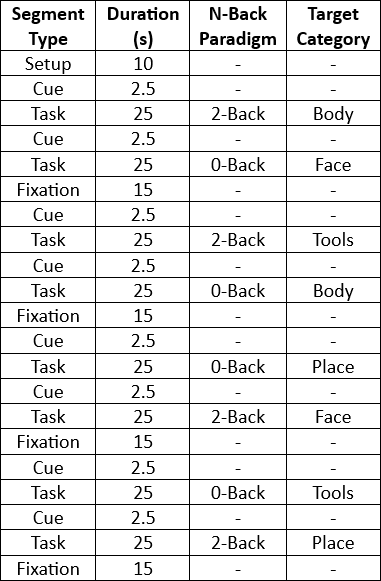
\includegraphics[width=0.4\textwidth]{assets/images/WM_mat.png}
    \caption[]{Display of the exact sequence of events during the \gls{WM}-task paradigm.}
    \label{tab:WM_mat}
\end{wrapfigure}

% Manually add to the List of Tables and lower list of figures counter.
\addtocounter{table}{1}
\addcontentsline{lot}{table}{\protect\numberline{\thetable}HCP WM Task Event Sequence}
\addtocounter{figure}{-1}

Stimuli were projected onto a computer screen behind the subject's head within the imaging chamber. The screen was viewed by a mirror positioned approximately \SI{8}{\centi\meter} above the subject's face. Participants were presented with blocks of trials that consisted of pictures of places, tools, faces and body parts (non-mutilated parts of bodies with no "nudity"). Within each run, the four different stimulus types were presented in separate blocks. Also, within each run, half of the blocks use a 2-Back \gls{WM}-task and half use a 0-Back \gls{WM}-task (as a working memory comparison). In short, in "N-Back" tasks participants are presented a sequence of stimuli one-by-one. For each stimulus, they need to decide if the stimulus currently being displayed, belongs to the same category as the one presented \textit{N} trials before. The factors that influence performance are not only the number \textit{N}, but also the speed of presentation and the size of the set of stimuli. A \SI{2.5}{\second} cue indicated the task type (and target for 0-Back) at the start of the block. Each of the two runs contained eight task blocks (10 trials of \SI{2.5}{\second} each, for \SI{25}{\second}) and four fixation blocks (\SI{15}{\second}). On each trial, the stimulus is presented for \SI{2}{\second}, followed by a \SI{500}{\milli\second} \gls{ITI}. The procedure is showcased in time order in \autoref{tab:WM_mat}.

The following event-related contrasts can potentially be generated between 2-Back and 0-Back tasks: 1) targets for the first are 2-Back repeats while for the second, they are targets that match the cue stimulus; 2) non-targets are novel items for the former and targets that do not match the cue stimulus for the latter; and 3) lures are 1-Back and 3-Back repeats for the 2-Back tasks and repeated stimuli that do not match the cue stimulus, for 0-Back tasks.

% Segway to MVPA
The task design outlined above is expected to reveal distinct patterns of behavior, performance, and consequently brain activation among subjects. While there will be considerable overlap in these patterns, analysis can isolate the unique aspects, resulting in consistent and distinguishable \gls{fMRI} signal from specific brain areas in response to category-specific stimuli. This pattern recognition and screening from the selection of patterns that stood out, could enable the classification of certain brain regions as more responsive and associated with processing specific types of information.

\section{Analysis of fMRI Signal} %maybe analysis tools section, subsection mvpa, classification

% Explaining the main elements manipulated during analyses.
In the analysis of \gls{fMRI} signals, the primary output is a samples-by-features data matrix, similar in structure to conventional table matrices with rows and columns. Each feature represents a voxel in the brain image, and their maximum number depends on the protocol used during the \gls{fMRI} scan, determined by the institution that collected the data, not by the data users. Samples are created based on the researcher's design of the analysis. Each vector of data over multiple voxels for a single sample is called a pattern, and each cell contains information that integrates the \gls{BOLD} signal data as well as the researcher's analysis parameters.

% From BOLD to statistical value.
The \gls{BOLD} signal captured by the \gls{fMRI} machine undergoes a series of processing steps unique to each analysis, resulting in varied outcomes. These outcomes are shaped by the researcher's choices, which are tailored to address the specific goals and inquiries of the research. These processing steps, which are detailed in \autoref{subs:stat}, replace the \gls{BOLD} in each cell of the data matrix with a statistical value that reflects both the signal's characteristics and the researcher's decisions.

% Multidimensional problem and attributes.
At first glance, a samples-by-features matrix might seem to represent a two-dimensional analysis, but it is far more intricate. Each cell may contain data points that incorporate a single or multiple \gls{EV}s meaning each data point can be a function of several variables rather than a constant for each voxel. Additionally, sample attributes can further increase the number of variables included. These attributes, which function as headers of either rows, columns or the entire table, include crucial information such as the target stimulus that produced the corresponding pattern, and the chunk to which the pattern belongs. Patterns from different chunks are considered independent of each other. Researchers may designate sample attributes differently based on logical assumptions, which can yield different practical conclusions and potentially increase the degrees of freedom in the analysis. Such a practice is shown in detail in \autoref{subs:ch_per_subj}. 

%Notably, another attribute which should be explained is that of ds.a.vol.mat affine matrix

% Introduction to COPEs.
Apart from technical decisions in data processing, the two main levers that can be manipulated are: 1) determining how many of the total \gls{EV}s provided by the experiment design to include in the analysis and whether some variables can be grouped together based on the desired effect; and 2) establishing the correlation between these \gls{EV}s.

\subsection{Univariate Pattern Analysis \textit{(UPA)}}

\gls{UPA} is a statistical approach used in neuroimaging to analyse brain activity data, particularly focusing on individual voxels. This method examines each voxel independently, assessing how its activity varies in response to different experimental conditions. Technically, \gls{UPA} measures the magnitude of an \gls{EV} correlation paradigm, otherwise known as the \gls{COPE} in each voxel independently. While \gls{UPA} can calculate the mean and standard deviation of the activation pattern for each voxel, either across varying conditions or over time, it does not provide information about the overall distribution behavior or the joint probability and correlations between voxels.

For example, consider analyzing brain activity during all 0-Back trials featuring a face as a stimulus, with the only \gls{EV} being the stimulus category. This analysis might show activation in both the \gls{V1} and the \gls{FFA} during these trials. However, it cannot conclusively determine that these areas are more responsive to this stimulus category. By averaging the signal for this case and for three other identical \gls{UPA}s with different stimulus categories, one might conclude that the \gls{V1} area, showing similar activation across all categories, is not involved in category-specific information processing but is generally activated when the subject observes anything. Nevertheless, this claim would be weak, as \gls{UPA} cannot distinguish what percentage of the signal magnitude is directly due to the stimulus category versus other factors.

\gls{UPA} is straightforward and widely used due to its simplicity and ease of interpretation. It is particularly useful when incorporating a temporal element into the assessment, as the calculations for a more complex analysis over time can become excessive. However, \gls{UPA} does not account for interactions between voxels, which can limit its ability to detect complex brain activity patterns and can lead to false or weak classification of brain activity patterns. Despite this limitation, \gls{UPA} remains a valuable tool for identifying localized brain responses and establishing a baseline for more complex analyses.

\subsection{Multivariate Pattern Analysis \textit{(MVPA)}}

% Technical stuff
\glsreset{MVPA}
A more suitable tool for complex analyses and deriving concrete, all-encompassing conclusions would be \gls{MVPA}. In the context of neuroimaging, \gls{MVPA} is an advanced analytical technique that decode intricate brain stimulation patterns by leveraging the joint probability distribution of voxel activities. It involves examining multidimensional probability functions that capture the interdependencies and correlations between multiple voxels simultaneously. By considering the multidimensional \gls{PDF}, MVPA can model the likelihood of observing specific activation patterns across a \gls{ROI}, thereby incorporating the covariance matrix to account for the pairwise correlations among voxels. This covariance structure enables the identification of distributed neural networks that co-activate in response to cognitive tasks.

% Can uncover complex relationships
More specifically, \gls{MVPA} examines the entire spatial pattern of voxel activations, enabling the decoding of cognitive states, perceptual experiences, or experimental conditions from the distributed patterns of brain activity. This method can uncover intricate patterns and relationships that reflect complex neural processes.

\begin{figure}[htbp]
    \centering
    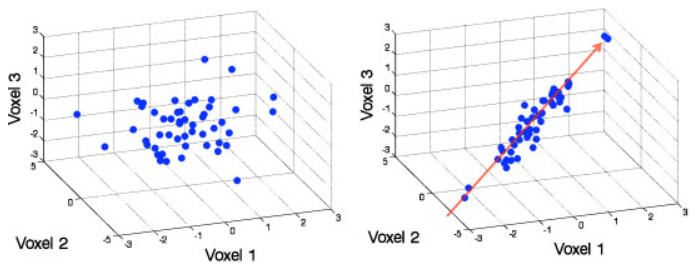
\includegraphics[width = 0.75\textwidth]{assets/images/Uni_vs_Multi.png}
    \caption[Illustration of the Difference Between MVPA and UPA]{Description of the difference between \gls{UPA} and \gls{MVPA}. On the left, there is no correlation between the three variables plotted, while on the right one can see a major source of variance indicating a positive correlation between all three voxels. A \gls{UPA} that just considered mean values on a voxel-to-voxel basis could not tell any difference between these two scenarios. In contrast, \gls{MVPA} identifies the sources of variance indicated by the red arrow before proceeding to construct neural activation patterns from these sources. Adapted from \paper{Habeck}{Habeck2010}.}
    \label{fig:UvsM}
\end{figure}

% Basis for classificaiton
At its core, \gls{MVPA} involves extracting patterns from \gls{fMRI} or other neuroimaging data and applying machine learning algorithms to classify these patterns. Common classifiers used in \gls{MVPA} include \gls{SVMs}, logistic regression, and neural networks, which can learn to distinguish between different cognitive states based on training data. By training these classifiers on labeled data, \gls{MVPA} can predict the cognitive state of new, unlabeled data with high accuracy. \gls{MVPA} also utilizes dimensionality reduction techniques like \gls{PCA} or \gls{ICA} to manage the high-dimensional nature of neuroimaging data, enhancing computational efficiency and reducing noise. Additionally, techniques like cross-validation are employed to ensure the robustness and reliability of the classifier’s predictions.

\clearpage

\subsection{Data Processing, Model Fitting and Classification}

\begin{figure}[htbp]
    \centering
    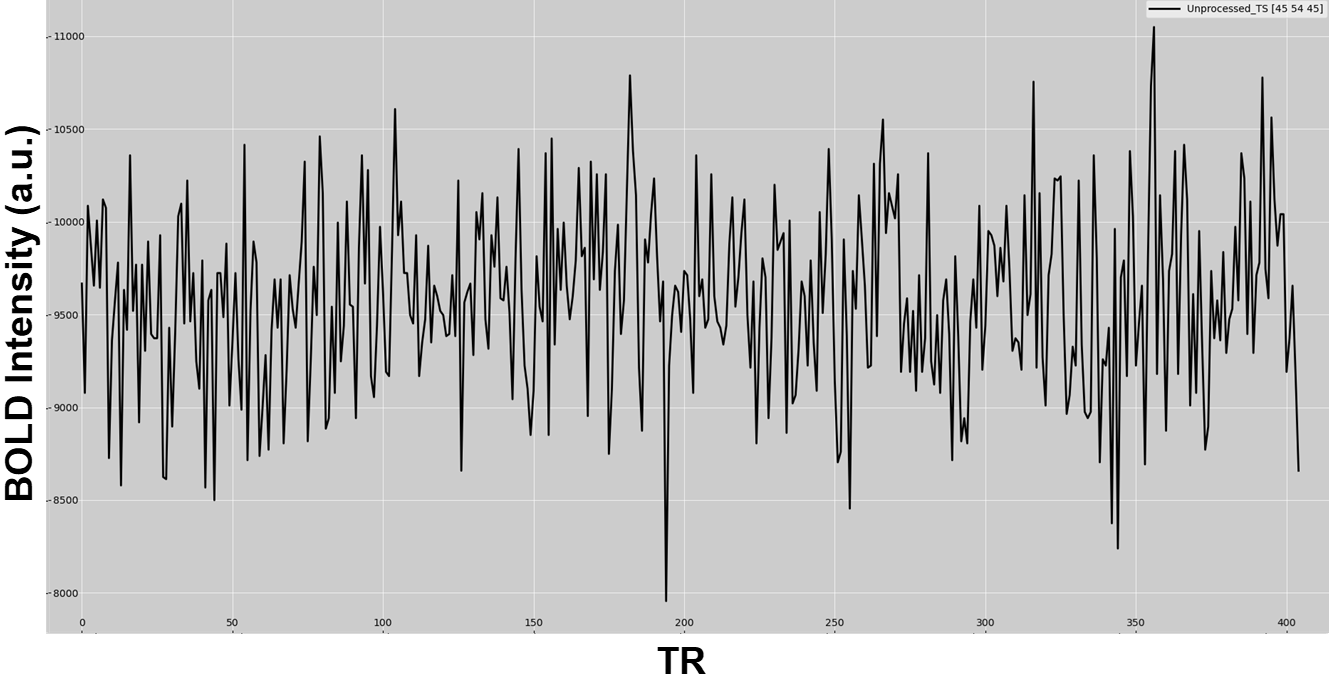
\includegraphics[width = 0.75\textwidth]{assets/images/unproc.png}
    \caption[Unprocessed Time-Series]{A snapshot of an unprocessed time-series.}
    \label{fig:Unp_TS}
\end{figure}

The unprocessed \gls{BOLD} signal is captured as a time-series (see \autoref{fig:Unp_TS}), representing the signal measured at each voxel throughout the entire \gls{fMRI} run. Initially, this unprocessed time series is quite ragged, featuring high resolution but also substantial noise, often to the point where noise overshadows the signal. To enhance the signal-to-noise ratio, several preprocessing steps are taken, including skullstripping \cite{Smith2002}, motion correction using rigid-body transformations, slice-timing correction, high-pass filtering, and, most importantly, smoothing. Smoothing involves replacing the signal at each voxel with a weighted average of its neighbors, which reduces spatial resolution but significantly improves the signal-to-noise ratio. This process also facilitates the normalization of the subject's brain to a template brain with standardized coordinates using affine transformations. Once preprocessing is complete, the time series appears as shown in \autoref{fig:P_TS}.

\begin{figure}[htbp]
    \centering
    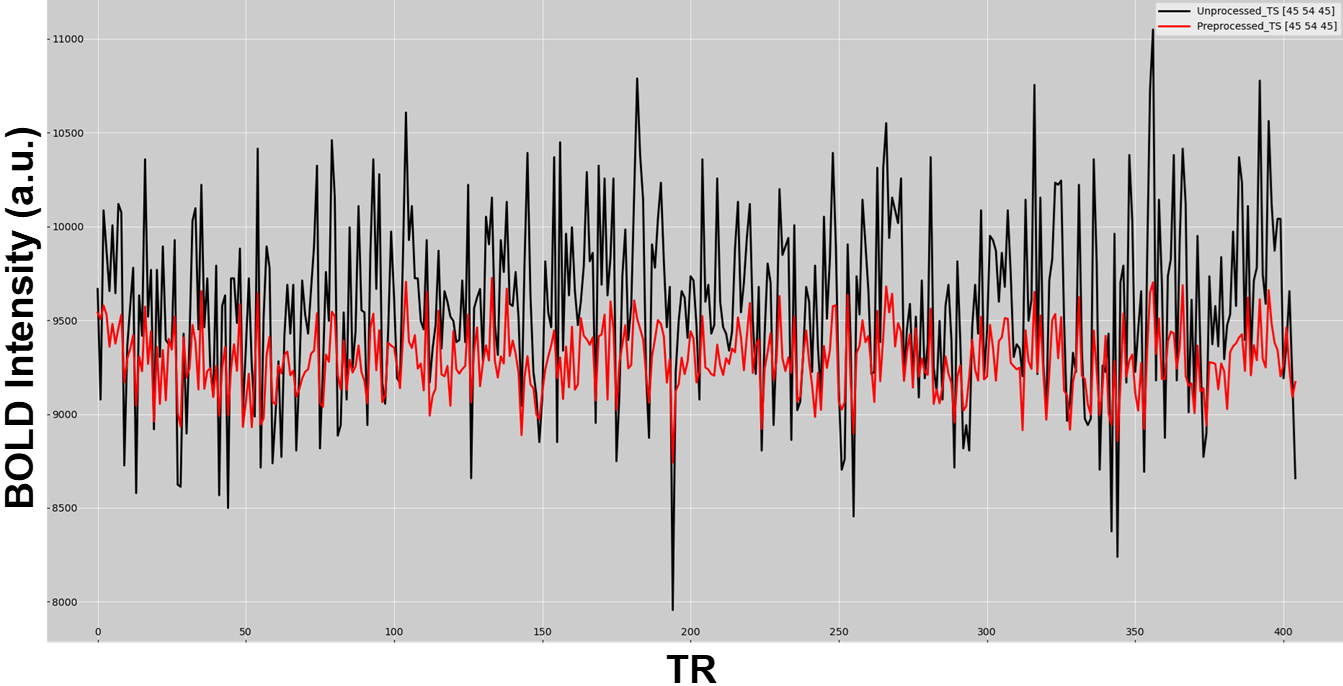
\includegraphics[width = 0.75\textwidth]{assets/images/preproc_and_unproc.png}
    \caption[Preprocessed Time-Series]{A snapshot of a pre-processed time-series.}
    \label{fig:P_TS}
\end{figure}

Now the time series is ready for model fitting. To achieve this, an assumption has to be made as to the expected form of the \gls{BOLD} response. Empirical studies \cite{Hirano2011, Martindale2003} demonstrated that, after a stimulus is presented, any responsive part of the brain exhibits an increase in \gls{BOLD} signal. This response typically follows a consistent pattern, peaking around \SI{6}{\second} and then returning to baseline over the next several \si{\second}. This shape can be modeled with a gamma distribution \cite{Andy_HRF}. When the gamma distribution is parameterized to best fit the observed \gls{BOLD} response observed by the majority of empirical studies, it is known as the canonical \gls{HRF}. The \gls{HRF} generated by a single impulse stimulus is illustrated in Figure \autoref{fig:single_HRF}, while the \gls{HRF} for a "boxcar" stimulus is shown in Figure \autoref{fig:box_HRF}.

\begin{figure}[htbp]
 	\centering
	\begin{subfigure}{0.49\textwidth}
		\centering
    		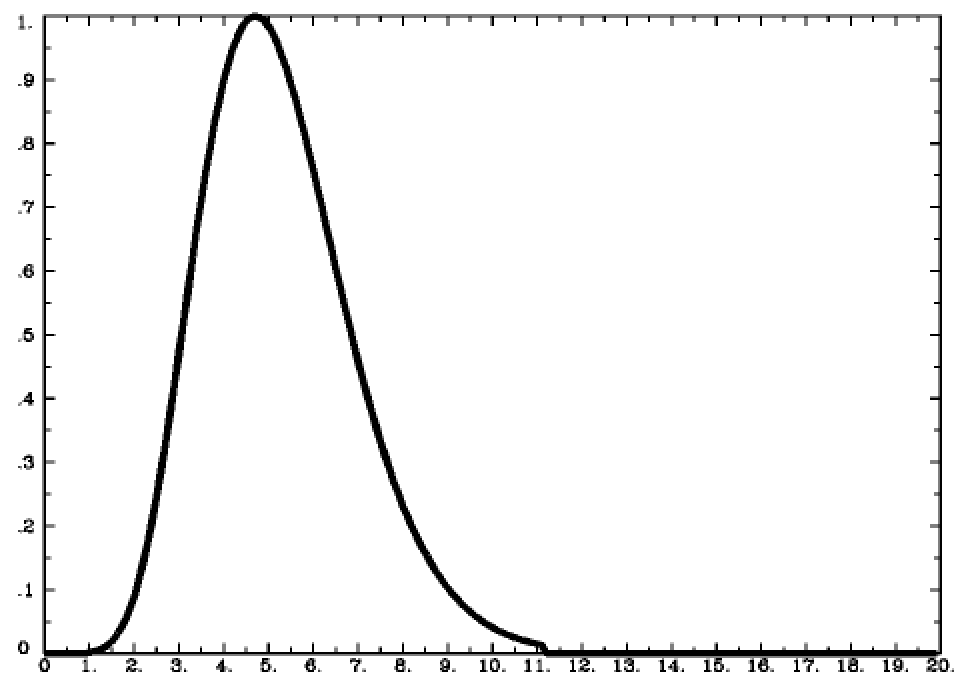
\includegraphics[width = 4cm, height = 3cm]{assets/images/single_HRF.jpg}
    		\caption{The \acrshort{HRF} generated by a single impulse stimulus. In this instance, the stimulus occurs at timepoint $ 0 $ on the x-axis.}
    		\label{fig:single_HRF}
	\end{subfigure}
	\hfill
	\begin{subfigure}{0.49\textwidth}
		\centering
   		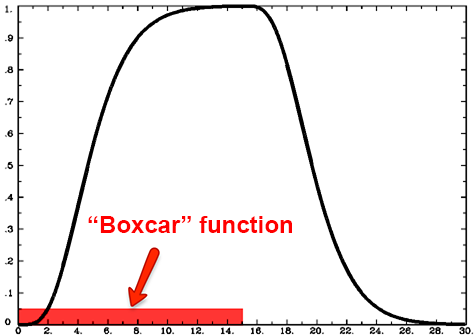
\includegraphics[width = 4cm, height = 3cm]{assets/images/box_HRF.jpg}
   		\caption{The \acrshort{HRF} generated by a "boxcar" stimulus lasting \SI{15}{\second}. Noteably, the \gls{BOLD} signal begins descending back to baseline around the \SI{15}{\second} mark.}
   		\label{fig:box_HRF}
	\end{subfigure}
	\caption[Fundamental HRF Shapes]{Illustration of the fundamental \gls{HRF} shapes. Adapted from \cite{Andy_HRF}.}
 	\label{fig:HRFs}
\end{figure}

Constructing a \gls{GLM} to fit the data involves estimating the expected \gls{BOLD} response by calculating the ideal beta weights for each regressor (\gls{EV}s). The model is then fitted to the time-series at each voxel, producing a function known as the fitted time-series, as shown in Figure \autoref{fig:fitted_TS}.

\begin{figure}[htbp]
    \centering
    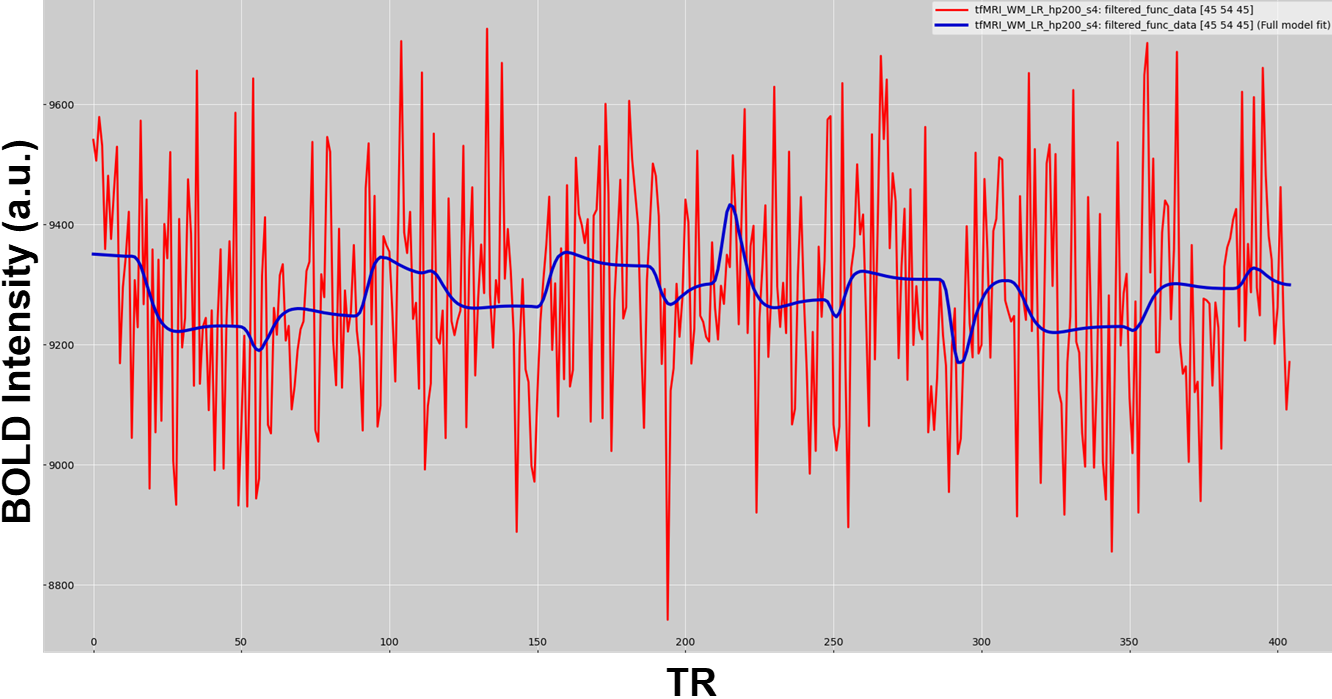
\includegraphics[width = 0.75\textwidth]{assets/images/fitted_and_preproc.png}
    \caption[Fitted Time-Series]{One instance of a fitted time-series, shown in red.}
    \label{fig:fitted_TS}
\end{figure}

This overarching \gls{HRF}, pertaining to one voxel and one \gls{COPE} (number of regressors) at a time, serves as the unit of data that can be fed into a classifier. It is these fitted time-series, or rather the beta-weights that characterize them, that the classifier trains on and eventually bases its predictions on.

% Details of fMRI image acquisition

%The \gls{HCP} structural acquisitions include high-resolution \gls{T1w} and \gls{T2w} images. Two separate averages of the \gls{T1w} image are acquired using the \acrshort{3D MPRAGE} (\cite{Mugler1990}) sequence with \SI{0.7}{\milli\meter} isotropic resolution (\acrshort{FOV} = \SI{224}{\milli\meter}, matrix = $320$, $256$ saggital slices in a single slab), \gls{TR} = \SI{2400}{\milli\second}, \gls{TE} = \SI{2.14}{\milli\second}, \gls{TI} = \SO{1000}{\milli\second}, \gls{FA} = $8^\circ$, \acrshort{BW} = \SI{210}{\hertz} per pixel, and \acrshort{ES} = \SI{7.6}{\milli\second}.








